\chapter{THIẾT KẾ GIẢI PHÁP}

\section{Giải pháp tổng quát}

\tab Để có được một công cụ xác định lỗi bảo mật web bằng các phương pháp khác nhau sẽ là một vấn đề rất rộng, cần nhiều thời gian cũng như nguồn lực mới có thể phát triển, triển khai và bảo trì.
Vì vậy, trong phạm vi của khóa luận, nhóm chọn thiết kế giải pháp dựa trên công cụ OWASP Zed Attack Proxy - ZAP là một công cụ mã nguồn mở uy tín trong giới, có đội ngũ chuyên môn cao và hàng trăm nhà phát triển đang đóng góp đến nay.
Các giải pháp nhóm đưa ra như sau.

\subsection{Giải pháp quét lỗi bảo mật với ZAP}

\tab Việc sử dụng ứng dụng ZAP trực tiếp sẽ đòi hỏi nhiều yêu cầu cần thiết như phần cứng đáp ứng đủ điều kiện sử dụng ứng dụng, lựa chọn phiên bản phù hợp với cấu hình, tải xuống, cài đặt môi trường (Java Runtime Environment - JRE), xử lý lỗi cài đặt - cấu hình.
Nhiều hơn nữa, để sử dụng được một số chức năng, người dùng cần phải biết cách cấu hình trình duyệt cho ZAP, quản lý dữ liệu của phiên sử dụng, cấu hình cho phương thức và nhiều tác vụ khác.
\par

Quét lỗi bảo mật web với ZAP là giải pháp, mục tiêu quan trọng và cốt lõi của hệ thống mà nhóm nhắm tới.
Với mục tiêu ban đầu là nhanh chóng, dễ sử dụng với mong muốn là dễ tiếp cận người dùng hơn thì các điều kiện đã nêu trên là vấn đề cần giải quyết.
Vì vậy, nhóm đề xuất giải pháp quét với bốn phương pháp có trong ZAP là Spider, Ajax Spider, Active và Passive là bốn phương pháp quét bảo mật web phổ biến và không cần sử dụng trực tiếp ứng dụng ZAP.
\par

Khi sử dụng giải pháp được đề xuất ở trên, người dùng có thể tạo các phiên quét bằng cách cung cấp các địa chỉ URL hoặc IP trang web cần quét và chọn các phương pháp quét.
Từ đó hệ thống sẽ thực hiện quét các phiên này với ZAP và thu được kết quả quét tương ứng của từng địa chỉ với từng phương pháp quét đã chọn.
Kết quả quét sẽ được lưu trữ, quản lý và hiển thị cho người dùng.
Với các phương pháp quét với Spider và Ajax Spider thì người dùng có thể xem được quá trình quét trong thời gian thực trong một số kịch bản nhất định.

\subsection{Giải pháp quản lý thông tin liên quan đến quá trình quét}

\tab Có các thông tin liên quan đến quá trình quét cần thiết được lưu trữ lại.
Vì vậy chúng em đề xuất 3 giải pháp kèm theo đó là quản lý là thông tin mục tiêu, thông tin lượt quét và quan trọng nhất là thông tin kết quả đã quét.

\subsubsection{Giải pháp quản lý mục tiêu}

\tab Để có quét một trang web ta cần xác định địa chỉ URL hoặc IP của trang web.
Trong phạm vi ứng dụng chúng em gọi các URL hay các IP này là “mục tiêu” để quét.
Cùng với đó, người dùng khi quét một mục tiêu thường sẽ có nhu cầu lưu và quản lý mục tiêu đó để dùng lại sau này.
Vì vậy đó cũng là lý do chúng em đưa ra giải pháp này.
\par

Một trong những chức năng tiên quyết của giải pháp này là thêm mới mục
Mục tiêu thêm mới sẽ cần các thông tin như tên mục tiêu, địa chỉ URL hay IP của mục tiêu và các nhãn dán mà người dùng muốn gán cho mục tiêu.
Có thể gán nhiều nhãn dán khác nhau cho một mục tiêu.
Các nhãn dán sẽ được đề xuất tự động khi người dùng đang thực hiện nhập thông tin tìm kiếm mục tiêu.
Các nhãn dán đề xuất được lấy dựa trên thông tin của các nhãn dán của những mục tiêu trước đó và các nhãn dán đề xuất sẽ không trùng nhau.
Các mục tiêu được quản lý sẽ sắp xếp bên dưới bảng với các cột chứa thông tin như tên, địa chỉ URL hay IP, nhãn, thời gian thêm và thời gian có thay đổi gần nhất.
Các mục tiêu trong bảng sẽ được sắp xếp theo thứ tự từ thời gian có thay đổi gần nhất đến thời gian có thay đổi xa nhất.
\par

Trong quá trình sử dụng, sẽ xuất hiện những mục tiêu người dùng không có nhu cầu sử dụng trong tương lai hay muốn làm gọn lại danh sách các mục tiêu.
Vì vậy, ứng dụng có chức năng xóa mục tiêu đã được tạo trước đó.
\par

Khi có danh sách các mục tiêu, để giúp cho người dùng tìm kiếm các mục tiêu thuận tiện hơn thì ứng dụng có chức năng tìm kiếm mục tiêu dựa theo tên của mục tiêu.
Khi sử dụng chức năng, mỗi khi người dùng nhập thông tin vào thanh tìm kiếm thì các mục tiêu có tên chứa thông tin đã nhập sẽ được lọc ra và các mục tiêu còn lại sẽ biến mất.
Người dùng cần xóa hết thông tin trong thanh tìm kiếm để có thể hiển thị lại toàn bộ các thông tin mục tiêu như cũ.
\par

Đồng thời, để cho việc bắt đầu phiên quét thuận tiện hơn, ứng dụng cũng có cung cấp chức năng bắt đầu quét trên mỗi mục tiêu.
Từ mục tiêu người dùng có thể chọn bắt đầu quét và được đưa đến màn hình lựa chọn loại quét và bắt đầu phiên quét như bình thường.
Rút ngắn bước cấu hình chọn lựa từng mục tiêu từ danh sách các mục tiêu trước khi cấu hình cho phiên quét.

\subsubsection{Giải pháp quản lý phiên quét và thông tin chi tiết kết quả quét}

\tab Trong giải pháp này, thông tin của từng phiên quét sẽ được quản lý dưới dạng bảng.
Bảng các phiên quét sẽ có các cột chứa các thông tin như tên mục tiêu, địa chỉ URL hay IP của mục tiêu, loại phương pháp quét, trạng thái quét, tiến độ quét và thời gian phiên quét được tạo và thời gian thông tin phiên quét được thay đổi gần nhất.
Các phiên quét trong bản sẽ được sắp xếp theo thứ tự thời gian có thay đổi gần nhất đến thời gian có thay đổi xa nhất.
\par

Khi trạng thái của các phiên quét đã hoàn thành thì người dùng có thể chọn vào phiên quét để đến màn hình thông tin chi tiết kết quả quét của phiên quét.
Tùy theo từng loại phương pháp quét của phiên quét thì thông tin chi tiết kết quả quét của phiên quét sẽ có cách hiển thị khác nhau.
Các thông tin về phiên quét cũng sẽ hiển thị trong màn hình này, các thông tin sẽ là mã định danh của phiên quét, cấu hình chi tiết tùy theo từng loại phương pháp quét và các thông tin hiển thị trên từng mục phiên quét ở bên ngoài bảng quản lý các phiên quét là tên mục tiêu, địa chỉ URL hay IP, loại phương pháp, trạng thái, tiến độ và các thời gian liên quan.
\par

Việc phải truy cập vào hệ thống và truy xuất thông tin chi tiết kết quả của phiên quét có thể sẽ gây khó khăn cho người dùng trong quá trình sử dụng nên ứng dụng có chức năng xuất tệp định dạng tài liệu di động (Portable Document Format, viết tắt là PDF).
Tệp này sẽ chứa các thông tin có trong màn hình thông tin chi tiết kết quả quét của phiên quét, tùy theo từng phương pháp quét khác nhau sẽ thì tệp sẽ có cấu trúc khác nhau.
\par

\section{Thiết kế hệ thống}

\subsection{Thiết kế kiến trúc hệ thống}
\begin{figure}[H]
      \centering
      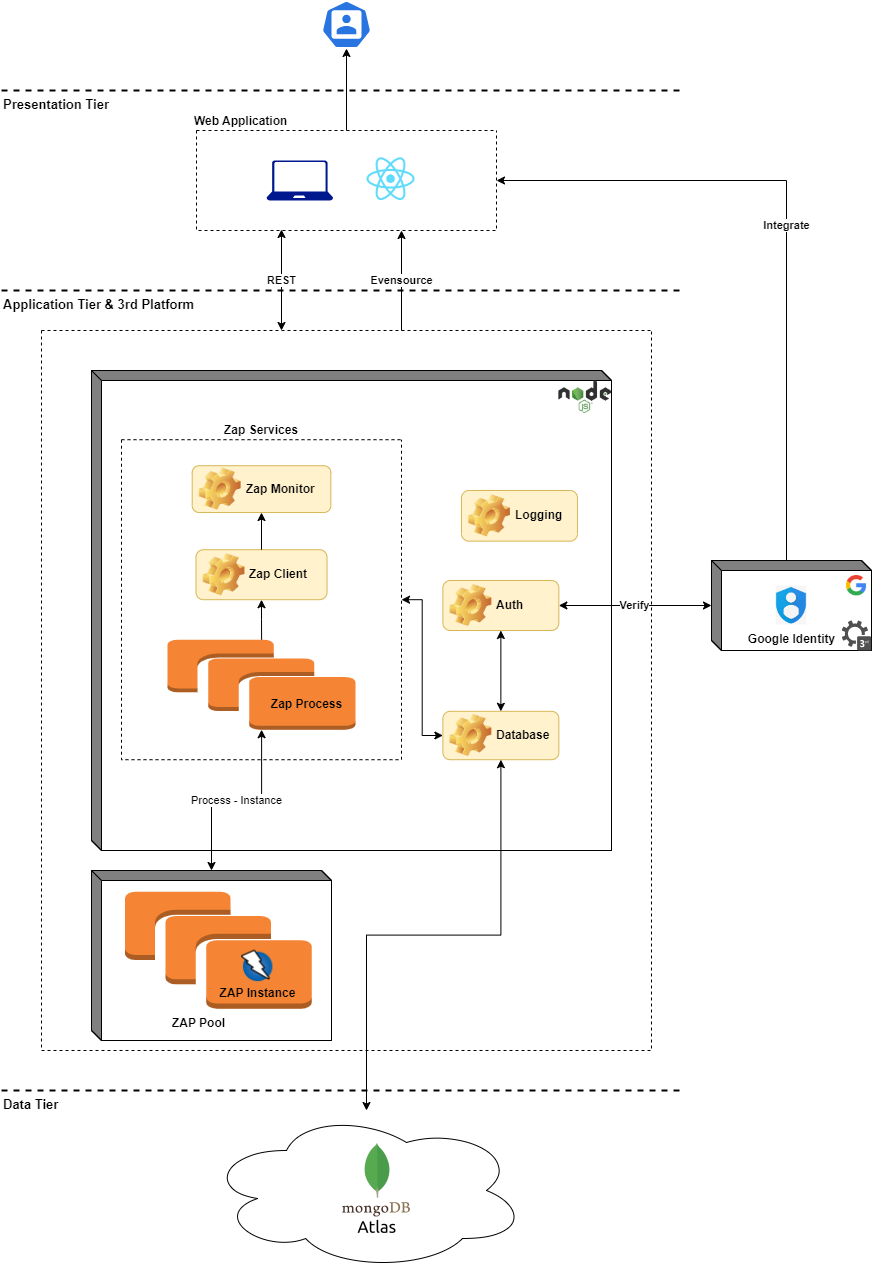
\includegraphics[width=\textwidth]{applied-thesis-chapters/chapter-3/Tổng quan kiến trúc hệ thống.png}
      \caption{Tổng quan kiến trúc hệ thống}
      \label{fig:KienTrucHeThong}
\end{figure}
\tab Hình số \ref{fig:KienTrucHeThong} thể hiện tổng quan kiến trúc hệ thống được xây dựng theo mô hình N-Tier đã đề cập ở chương 2.x.x.
Kiến trúc hệ thống gồm 3 tầng (3-Tier): Tầng trình bày, tầng ứng dụng và tầng dữ liệu.

\subsubsection{Thiết kế kiến trúc hệ thống tầng trình bày}

\tab Tầng trình bày (Presentation tier) là tầng ứng dụng web phục vụ cho người dùng.
Người dùng tương tác trên giao diện ứng dụng web để tiếp cận với các giải pháp mà nhóm đã đề cập đến ở chương 3.1.
Theo như kiến trúc, ứng dụng của tầng trình bày được xây dựng chính bằng thư viện React và các công cụ có hỗ trợ React.

\subsubsection{Thiết kế kiến trúc hệ thống tầng ứng dụng}

\tab Tầng ứng dụng (Application tier) là tầng có trách nhiệm xử lý đa phần mọi giải pháp của hệ thống, là tầng chính của toàn bộ hệ thống.
Theo như kiến trúc, tầng ứng dụng chứa hai phần là ứng dụng chính và tập hợp các đối tượng ZAP (ZAP Pool).
\par

Ứng dụng chính bao gồm các dịch vụ (service) được cài đặt tách biệt với nhau, mang nhiệm vụ riêng để tăng tính trực quan và linh hoạt, khả năng mở rộng và bảo trì, tránh các lỗi xung đột không đáng có, dễ dàng phát triển và tích hợp.
Các service bao gồm: nhóm các ZAP service, dịch vụ xác thực (Authentication service), dịch vụ cơ sở dữ liệu (Database service) và dịch vụ ghi nhật ký (Logging service).
\par

\myparagraph{Nhóm ZAP service}
\tab \tab Nhóm các ZAP service bao gồm hai service chính là dịch vụ quản lý ZAP (ZAP Monitor service) và dịch vụ tương tác với ứng dụng ZAP (ZAP Client service), cuối cùng là lớp tiến trình ZAP (ZAP Process).
Hình \ref{fig:NhomZapServiceHoatDong} sẽ cho ta cái nhìn chi tiết hơn về cách hoạt động của nhóm ZAP service trong hệ thống.

\begin{figure}[H]
      \centering
      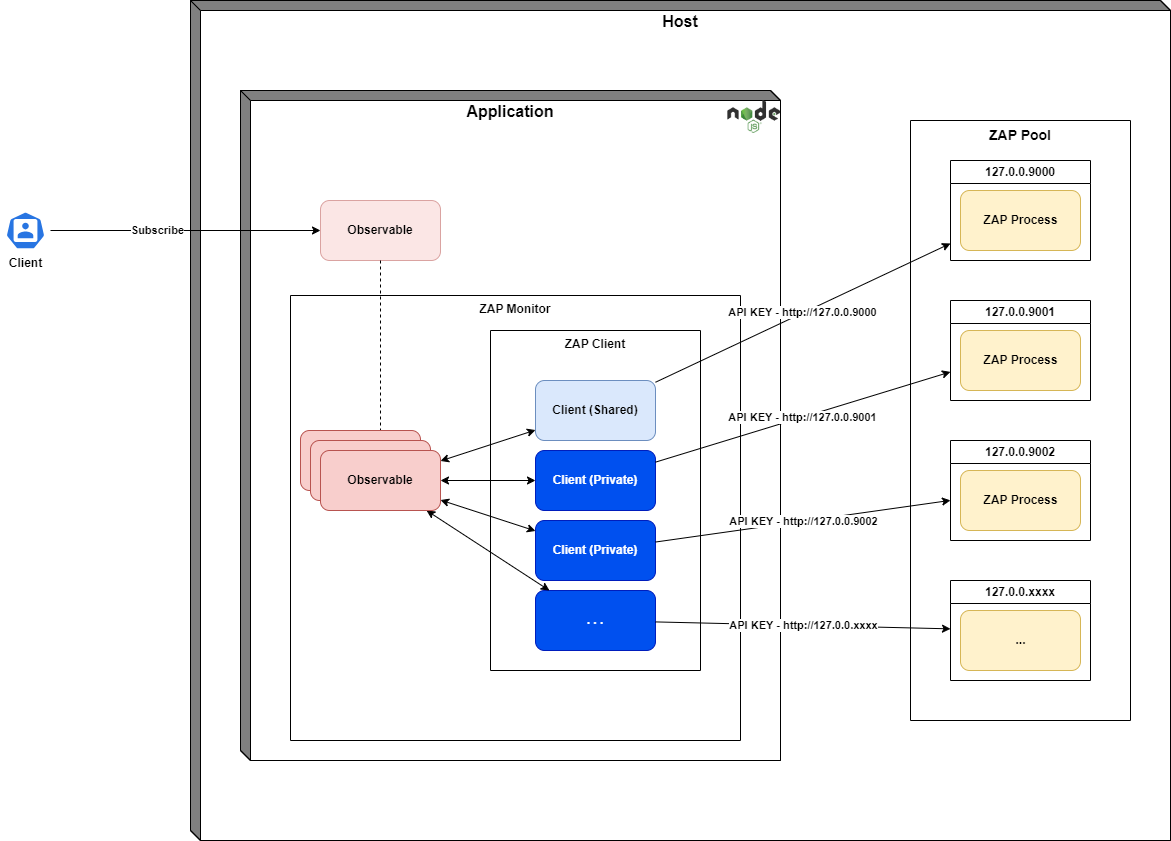
\includegraphics[width=\textwidth]{applied-thesis-chapters/chapter-3/Mô tả nhóm ZAP service hoạt động trong hệ thống.png}
      \caption{Mô tả nhóm ZAP service hoạt động trong hệ thống}
      \label{fig:NhomZapServiceHoatDong}
\end{figure}

\begin{itemize}
      \item \textbf{ZAP Process:} Mỗi tiến trình ZAP sẽ được khởi tạo từ lớp ZAP Process, gọi là ZAP Process instance.
            Mỗi instance là process chạy ngầm trong hệ thống (trình nền - daemon).
            Các instance này hoạt động lập với nhau trên các cổng (port) khác nhau như một ứng dụng được khởi chạy riêng biệt.
      \item \textbf{ZAP Client service:} Service có nhiệm vụ tạo và quản lý các ZAP client.
            Mỗi ZAP client được service quản lý qua một mã định danh duy nhất (UUID - Universally Unique Identifier) và tham chiếu đến mỗi ZAP Process instance khác nhau.
            ZAP client có vai trò tương tác, điều khiển ZAP process thực hiện các tác vụ của ZAP qua phương thức HTTP.
            Vì ZAP process chỉ là một process chạy ngầm trong hệ thống và tách biệt với ứng dụng chính nên ZAP Client service là một trong những service quan trọng của ứng dụng chính.
            Theo như giải pháp thì mỗi phương pháp quét sẽ cần mỗi ZAP process có hành vi, cấu hình khác nhau.
            Nhóm chia thành hai loại là:
            \begin{itemize}
                  \item \textbf{ZAP Client Shared:} Client này dành cho các phương pháp quét có thể sử dụng chung ZAP process instance, kết quả các phiên quét tuy sử dụng chung instance nhưng không ảnh hưởng đến nhau.
                        Cặp client shared và ZAP process và luôn luôn tồn tại xuyên suốt quá trình sống của ứng dụng
                  \item \textbf{ZAP Client Private:} Client này dành cho các phương pháp quét không thể sử dụng chung ZAP process instance.
            \end{itemize}
      \item \textbf{ZAP Monitor service:} Service có vai trò đại diện cho nhóm ZAP service.
            Cài đặt của các giải pháp của ứng dụng chính chỉ giao tiếp với service này.
            Service có nhiệm vụ tạo, dừng và quản lý các phiên quét của người dùng; nắm giữ và quản lý quá trình quét của các phiên quét, giúp cho hệ thống có thể kết nối và biết được các thông tin về trạng thái và tiến độ của phiên quét; lưu trữ các dữ liệu cần thiết khi hoạt động với ZAP như thông tin phiên quét, thông tin kết quả với Database service.
\end{itemize}

\myparagraph{ZAP Pool}
\tab \tab Là tập hợp các ZAP process instance chạy ngầm, mỗi instance sẽ chạy trên một cổng (port) khác nhau và được tham chiếu bởi các ZAP client của ZAP Client service.
\par

Hình \ref{fig:TTZapMonitorStartScan} và \ref{fig:TTHeThongStartScan} thể hiện quá trình tương tác và hoạt động của nhóm ZAP service trong hệ thống khi bắt đầu một phiên quét.

\begin{figure}[H]
      \centering
      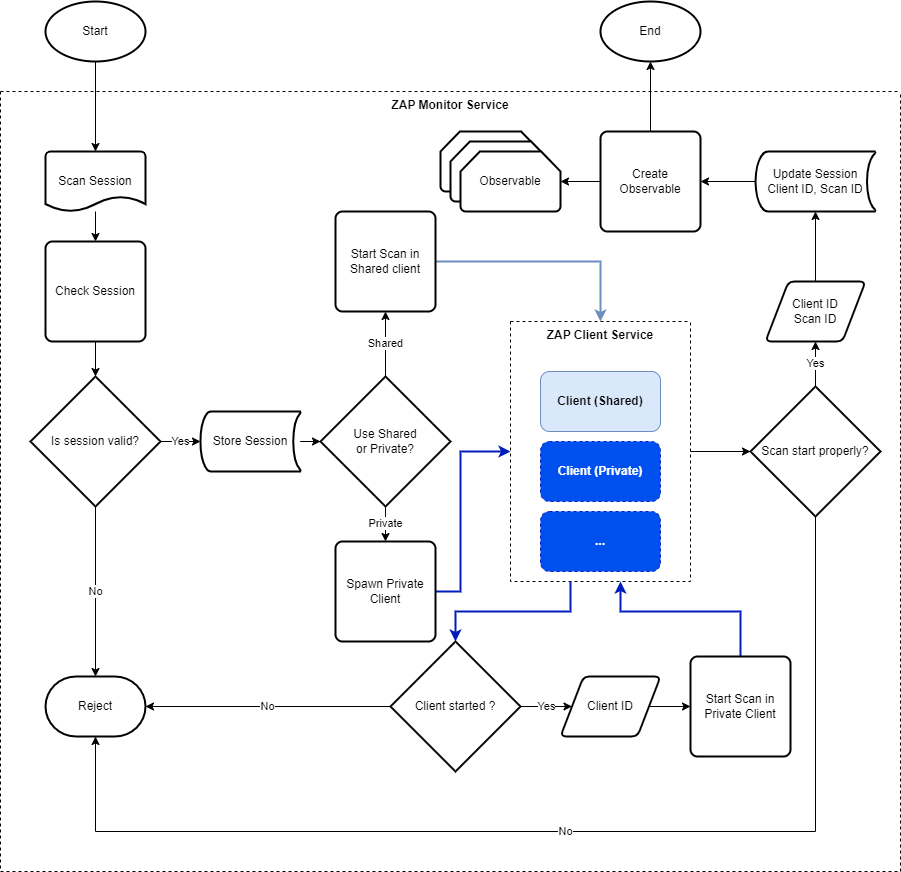
\includegraphics[width=\textwidth]{applied-thesis-chapters/chapter-3/Sơ đồ tuần tự của quá trình bắt đầu phiên quét của ZAP Monitor service.png}
      \caption{Sơ đồ tuần tự của quá trình bắt đầu phiên quét của ZAP Monitor service}
      \label{fig:TTZapMonitorStartScan}
\end{figure}

\begin{figure}[H]
      \centering
      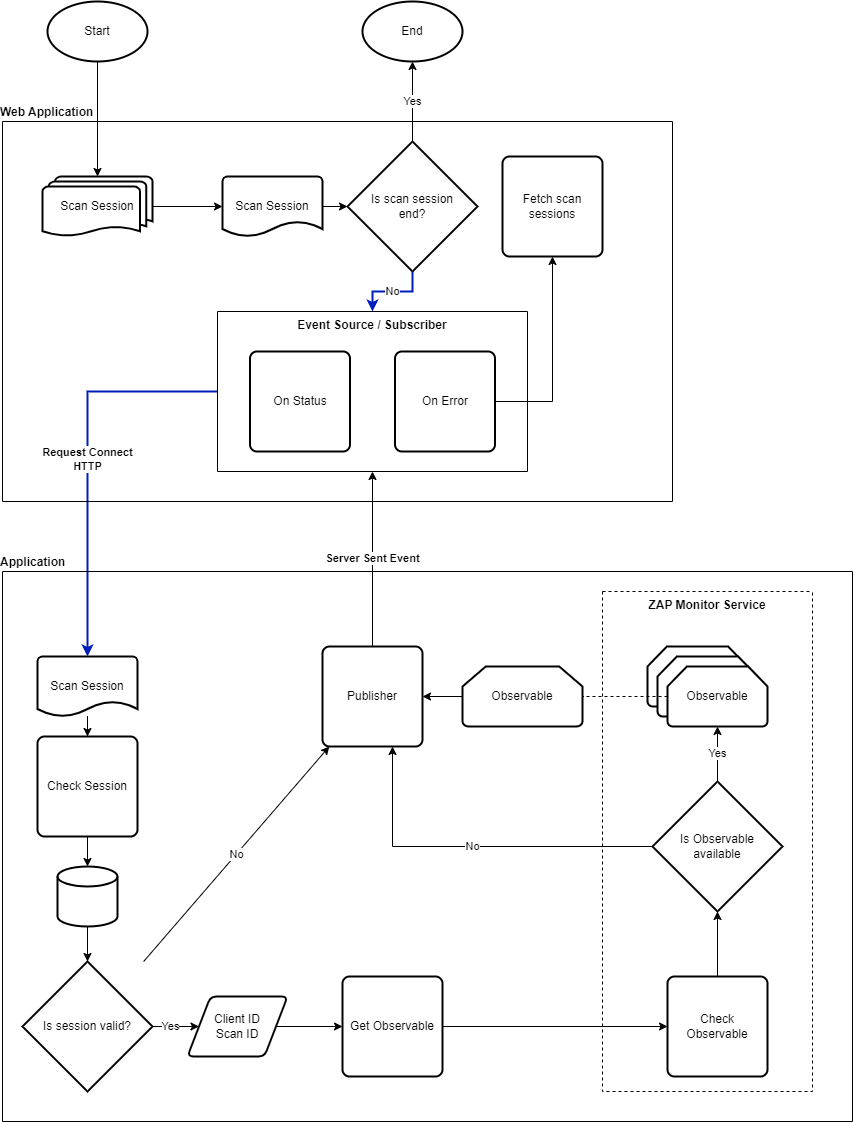
\includegraphics[width=\textwidth]{applied-thesis-chapters/chapter-3/Sơ đồ tuần tự của quá trình bắt đầu phiên quét của hệ thống với ứng dụng web.png}
      \caption{Sơ đồ tuần tự của quá trình bắt đầu phiên quét của hệ thống với ứng dụng web}
      \label{fig:TTHeThongStartScan}
\end{figure}

\myparagraph{Authentication service}
\tab \tab Service thực hiện các nhiệm vụ liên quan đến xác thực người dùng.
Các nhiệm vụ như xác minh lại token nhận được từ ứng dụng web từ bên thứ ba là Google Identify, đọc ghi dữ liệu người dùng với Database service.

\myparagraph{Logging service}
\tab \tab Service có trách nhiệm ghi lại nhật kí (log) cho toàn bộ ứng dụng, bao gồm cả các ZAP process chạy ngầm.
Vì các ZAP process được chạy ngầm nằm ngoài phạm bị của ứng dụng và nhu cầu lấy log của các process này là cần thiết nên service này được cài đặt.
Log của các service khác nhau được phân biệt bằng tên loại khác nhau, các tên này được sử dụng là tiền tố khi hiển thị trong bảng điều khiển (console).
Chủ yếu có bốn loại log hiện có trong ứng dụng là:

\begin{itemize}
      \item \textbf{Main process log:} Các log này trình bày các tác vụ, lỗi phát sinh bên trong ứng dụng chính, đa phần nằm trong ZAP Monitor service.
      \item \textbf{Http request log:} Các log này trình bày thông tin chi tiết các yêu cầu (request) được gửi đến ứng dụng ở mọi tuyến (route).
      \item \textbf{User session process log:} Các log này trình bày thông tin các kết nối của người dùng với các phiên quét.
            Mỗi phiên quét sẽ có quá trình quét, các quá trình quét sẽ được quản lý bởi ZAP Monitor service, thông tin của phiên quét là trạng thái và tiến độ sẽ được gửi đến người dùng theo thời gian thực (stream).
            Thông tin các kết nối stream của người dùng sẽ được ghi lại trong loại log này.
      \item \textbf{ZAP process log:} Log này được nhúng vào mỗi ZAP process khi chúng vừa được khởi tạo.
            Các log này trình bày thông tin của chính ZAP process đó in ra trong console của nó.
            Theo như nghiệp vụ của giải pháp, loại log này còn có một biến thể nữa là ZAP private process log.
            ZAP process log bình thường sẽ ghi lại các log trong ZAP shared process instance, còn ZAP private process log sẽ ghi lại các log trong các ZAP private process instance.
\end{itemize}

\myparagraph{Database service}
\tab \tab Service có nhiệm vụ là kết nối với MongoDB Atlas và đại diện thực hiện các thao tác đọc ghi, truy vấn với cơ sở dữ liệu đã kết nối.

\subsubsection{Thiết kế kiến trúc hệ thống tầng dữ liệu}

\tab Tầng dữ liệu là tầng cơ sở dữ liệu, nơi các dữ liệu của hệ thống được lưu trữ.
Các dữ liệu được lưu trữ trong hệ thống là thông tin định danh người dùng, các dữ liệu liên quan đến mục tiêu và phiên quét.
\par

Cơ sở dữ liệu MongoDB là một cơ sở dữ liệu hướng tài liệu, thuộc dạng cơ sở dữ liệu phi quan hệ (NoSQL).
Bản ghi dữ liệu trong MongoDB được ghi đệm (cache) lên RAM (Random Access Memory) khi có truy vấn đến nó, hạn chế truy cập vào ổ cứng nên tốc độ đọc ghi cao.
\par

Nhóm đề xuất sử dụng MongoDB làm cơ sở dữ liệu do các tính chất trên phù hợp với giải pháp ứng dụng.
Giải pháp ứng dụng yêu cầu ghi nhiều loại dữ liệu có cấu trúc linh hoạt, đa dạng.
Các dữ liệu có cấu trúc linh hoạt tiêu biểu như:

\begin{itemize}
      \item Bản ghi cấu hình và kết quả của phiên quét của các phương thức quét khác nhau.
      \item Bản ghi thông tin phiên quét trong quá trình quét cần đọc ghi nhiều lần.
\end{itemize}

Tiếp theo, như đã nhắc đến ở trên, bản ghi dữ liệu của MongoDB có thể cache lên RAM để tăng tốc truy vấn dữ liệu và mặc định sử dụng 50% RAM trên hệ thống.
Cùng với việc hệ thống thường phải hoạt động với cường độ cao, sử dụng 80 đến 90% hiệu suất Bộ xử lý trung tâm (Central Processing Unit, viết tắt là CPU) và 60 đến 70% hiệu suất RAM, khi thực hiện nhiều phiên quét cùng lúc. 
Vậy nên rủi ro dữ liệu không được ghi một cách đúng đắn khi hệ thống hoạt động hiệu suất cao là có tồn tại.
\par

Để giải quyết vấn đề này, nhóm đề xuất sử dụng MongoDB Atlas là một dịch vụ cơ sở dữ liệu đám mây (cloud database service).
MongoDB Atlas là một cloud database dành riêng và thuộc sự quản lý trực tiếp của MongoDB.
Về bản chất, database được triển khai hoàn toàn trên VPC là Google Cloud Platform, AWS hay Microsoft Azure dựa theo tùy chọn khi khởi tạo.
Người dùng có thể kết nối, quản lý, tương tác qua trung gian MongoDB Atlas.
Như hình \ref{fig:KetNoiAtlas}, ứng dụng chính tương tác với database trên VPC bằng trình điều khiển MongoDB (MongoDB driver) qua phương thức TCP/IP socket.
\par

\begin{figure}[H]
      \centering
      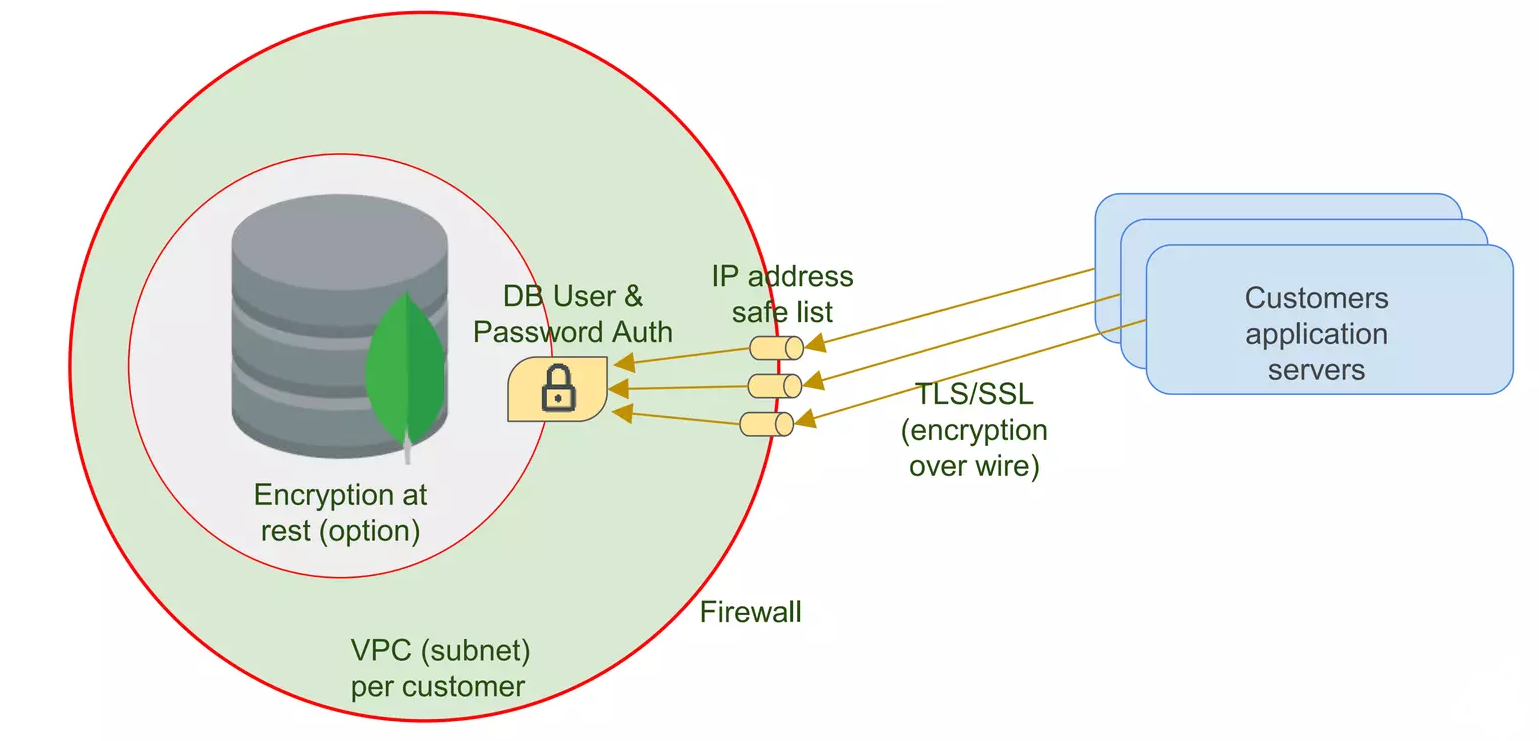
\includegraphics[width=\textwidth]{applied-thesis-chapters/chapter-3/Mô tả kết nối của ứng dụng với MongoDB Atlas.png}
      \caption{Mô tả kết nối của ứng dụng với MongoDB Atlas}
      \label{fig:KetNoiAtlas}
\end{figure}

Về cơ bản, nhóm triển khai MongoDB trên một máy dịch vụ khác, không triển khai chung với hệ thống để tránh các vấn đề hiệu suất hệ thống ảnh hưởng đến toàn vẹn dữ liệu.
Chuyển sự hạn chế bởi cấu hình của MongoDB sang máy khác nghĩa là không còn giữ nguyên được tính nhanh chóng (cache) và các tương tác với database phải thông qua giao thức TCP/IP socket (chức năng cache vẫn hoạt động bình thường ở VPC).
Bên cạnh lợi ích toàn vẹn dữ liệu, việc lựa chọn giải pháp này cũng mang lại nhiều lợi ích khác như tăng tính bảo mật, mở rộng, linh hoạt, tiện lợi, dễ dàng quản lý và không cần nhiều bận tâm về các vấn đề của database trên hệ thống chính.

\subsection{Thiết kế giao diện hệ thống}

\subsubsection{Giao diện trang chủ}

\tab Màn hình trang chủ là nơi người dùng sẽ tiếp cận đầu tiên khi truy cập vào tên miền gốc của ứng dụng.
Màn hình có hai thành phần chính là giới thiệu chung về ứng dụng và phần cho phép người dùng sử dụng thử chức năng quét với phương thức Spider, không cần đăng nhập xác minh.
Giao diện màn hình trang chủ được thiết kế như sau, hình \ref{fig:MHTrangChu}:

\begin{figure}[H]
      \centering
      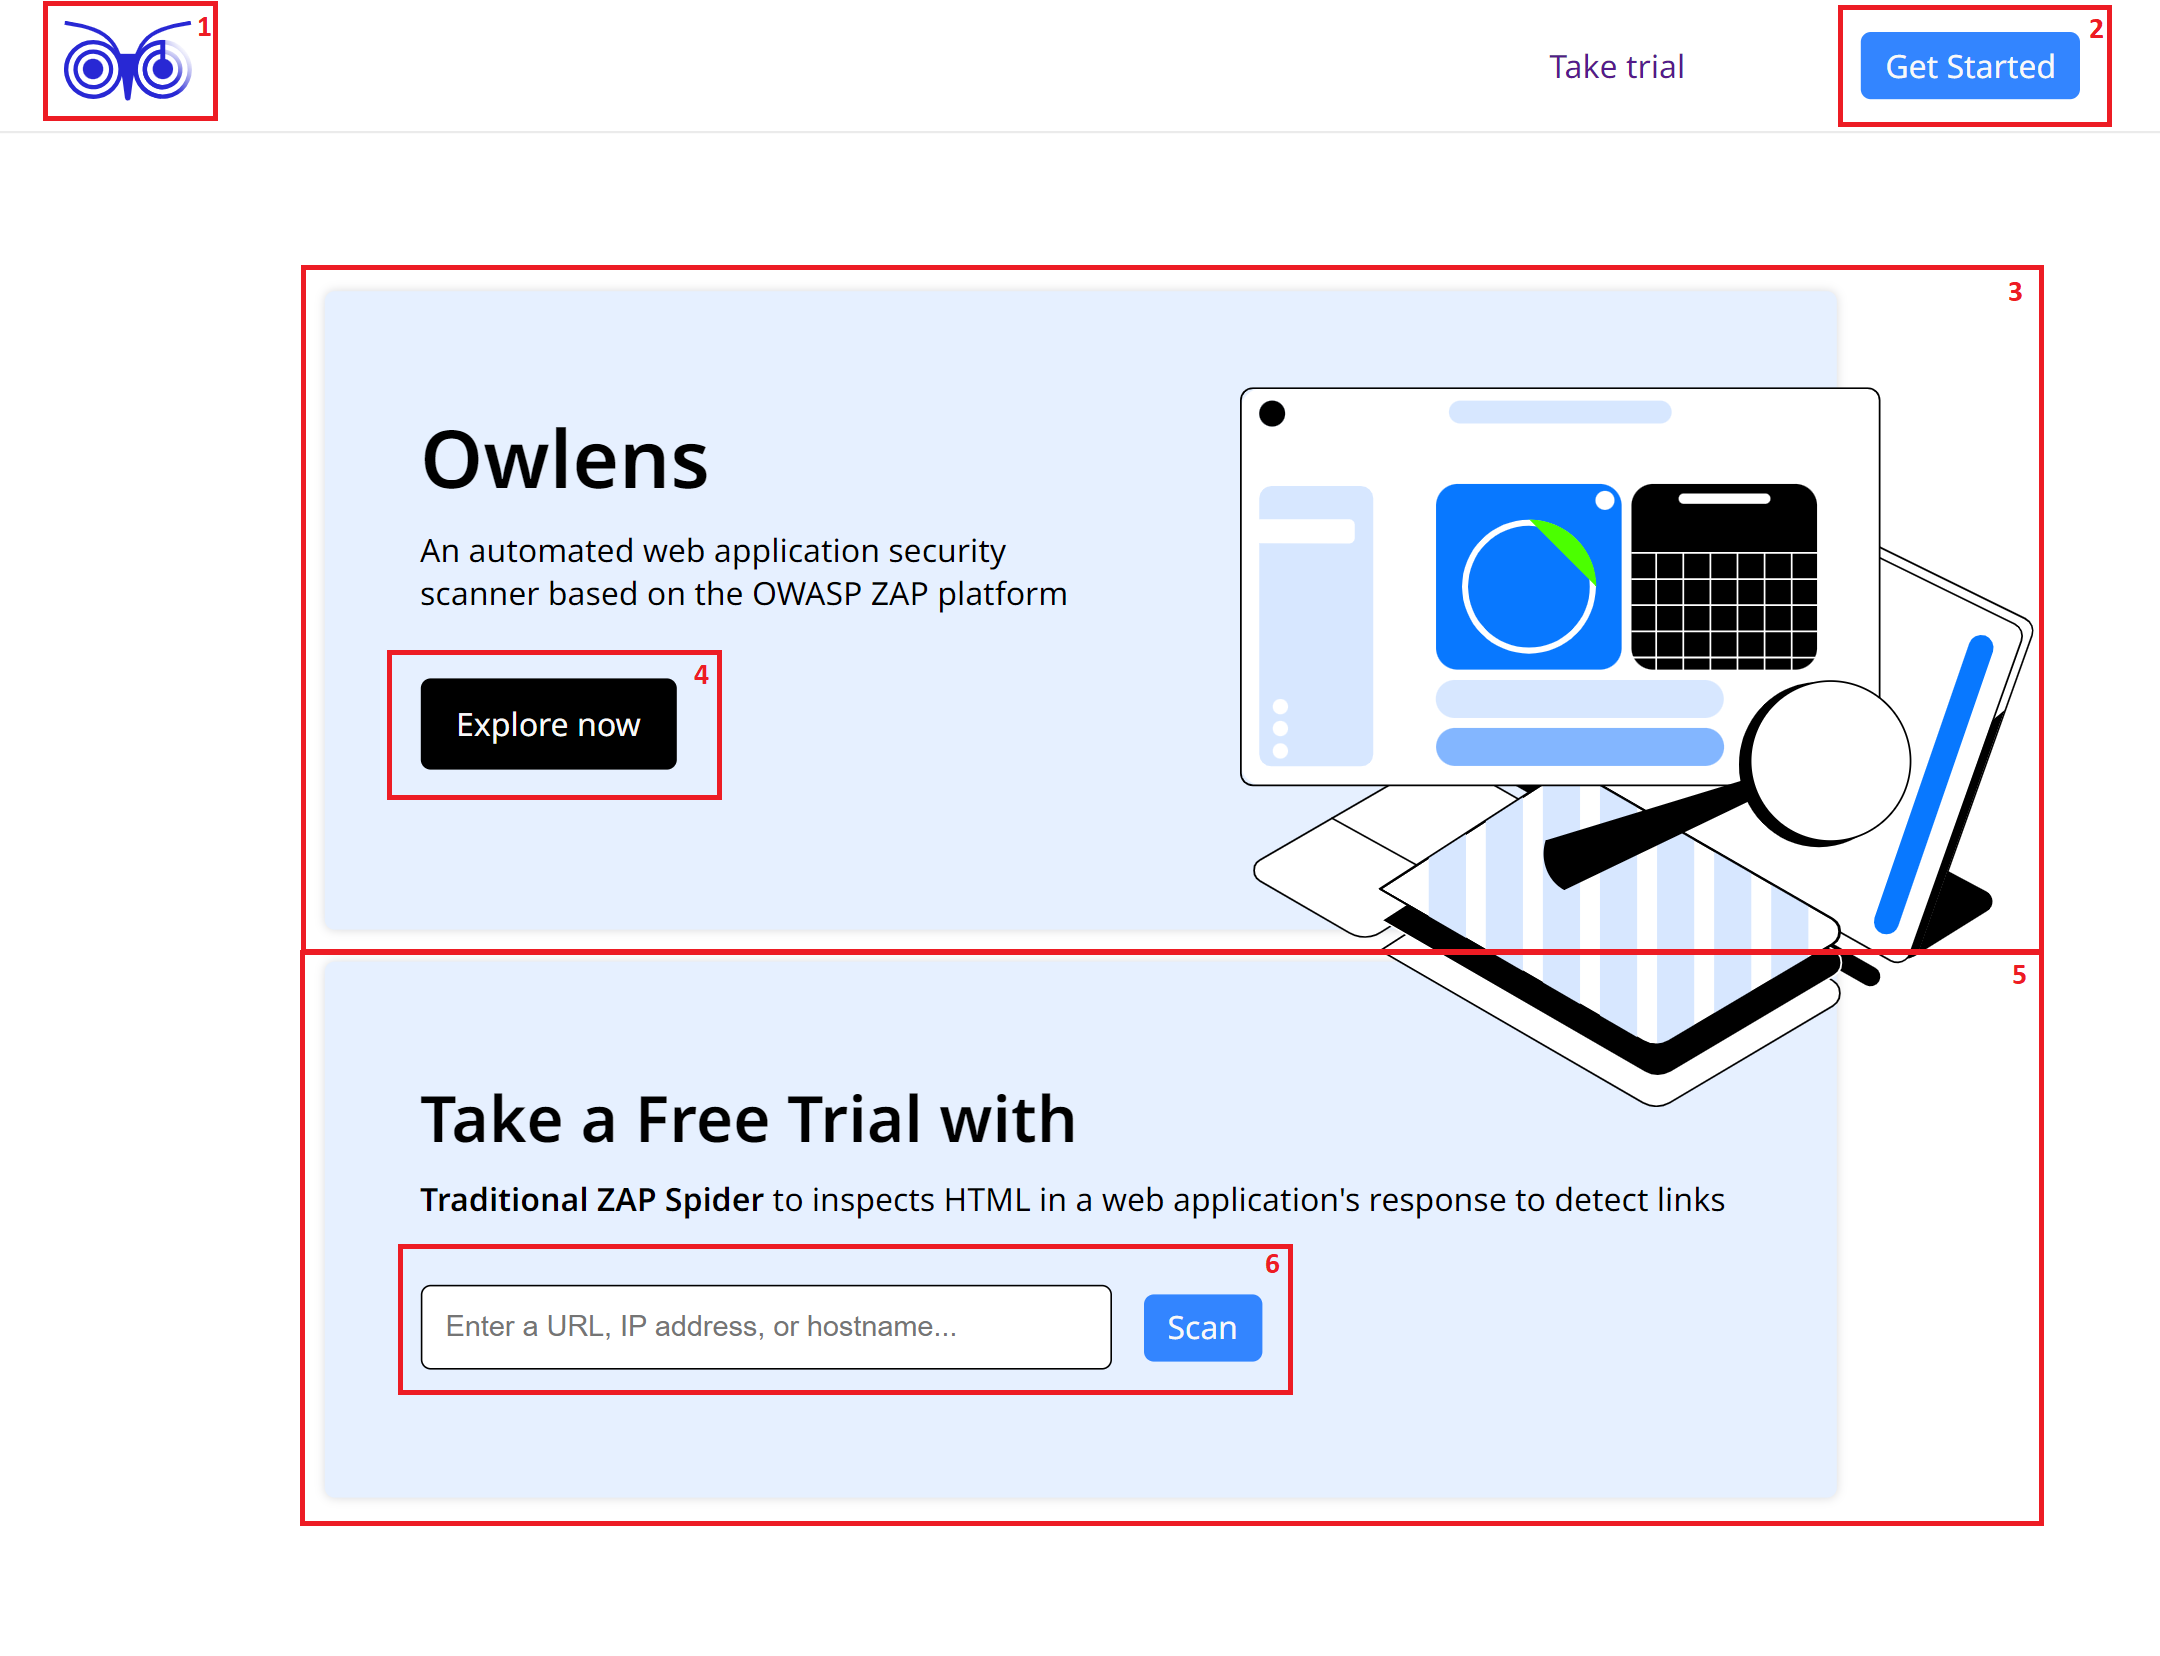
\includegraphics[width=\textwidth]{applied-thesis-chapters/chapter-3/Màn hình trang chủ.png}
      \caption{Màn hình trang chủ}
      \label{fig:MHTrangChu}
\end{figure}

Bảng mô tả giao diện màn hình trang chủ, bảng \ref{tab:MTTrangChu}:

\begin{tabularx}{\textwidth}{|>{\hsize=.15\hsize\centering\let\newline
      \\\arraybackslash}X|>{\hsize=.30\hsize\raggedright\let\newline
      \\\arraybackslash}X|>{\hsize=.45\hsize\raggedright\let\newline
      \\\arraybackslash}X|}
      \hline
      \thead{STT}
       & \thead{Tên thành phần}
       & \thead{Mô tả}
      \\
      \hline
      1
       &
      Logo
       &
      Logo của ứng dụng Owlens. Có thể chọn vào logo để điều hướng quay lại màn hình trang chủ.
      \\
      \hline
      2
       &
      Nút bắt đầu
       &
      Dùng để điều hướng đến trang đăng nhập và đăng ký của hệ thống.
      \\
      \hline
      3
       &
      Phần giới thiệu
       &
      Phần này giới thiệu thông tin, chức năng chung của hệ thống.
      \\
      \hline
      4
       &
      Nút gọi hành động (Call to Action, viết tắt là CTA)
       &
      Dùng để điều hướng đến trang đăng nhập và đăng ký của hệ thống.
      \\
      \hline
      5
       &
      Phần giới thiệu dùng thử
       &
      Giới thiệu thông tin phần dùng thử. Người dùng có thể sử dụng thử chức năng quét với phương thức Spider mà không cần đăng nhập xác minh.
      \\
      \hline
      6
       &
      Phần dùng thử
       &
      Người dùng dùng thử bằng cách nhập URL hoặc IP và chọn nút “Scan“ để bắt đầu phiên quét. Kết quả quét sẽ được hiển thị trực tiếp theo thời gian thực ngay trên cùng màn hình trang chủ, trong phần dùng thử. Vì không cần xác minh nên đối với kết quả quét xong, kết quả sẽ biến mất khi người dùng di chuyển ra khỏi màn hình trang chủ. Đối với kết quả đang được hiển thị trực tiếp, đang trong quá trình quét thì kết quả sẽ biến mất khi người dùng di chuyển quá 60 giây khỏi màn hình trang chủ.
      \\
      \hline
      \caption{Mô tả giao diện màn hình trang chủ}
      \label{tab:MTTrangChu}
\end{tabularx}

\subsubsection{Giao diện ứng dụng web}

\tab Màn hình ứng dụng web là nơi người dùng sẽ tiếp cận sau khi đăng nhập vào ứng dụng.
Màn hình này là nơi người dùng thực hiện hầu hết mọi tác vụ có trong ứng dụng.
Màn hình có hai thành phần chính là bảng tùy chọn và bản điều khiển.
Giao diện ứng dụng web được thiết kế như sau, hình \ref{fig:MHUngDung}:

\begin{figure}[H]
      \centering
      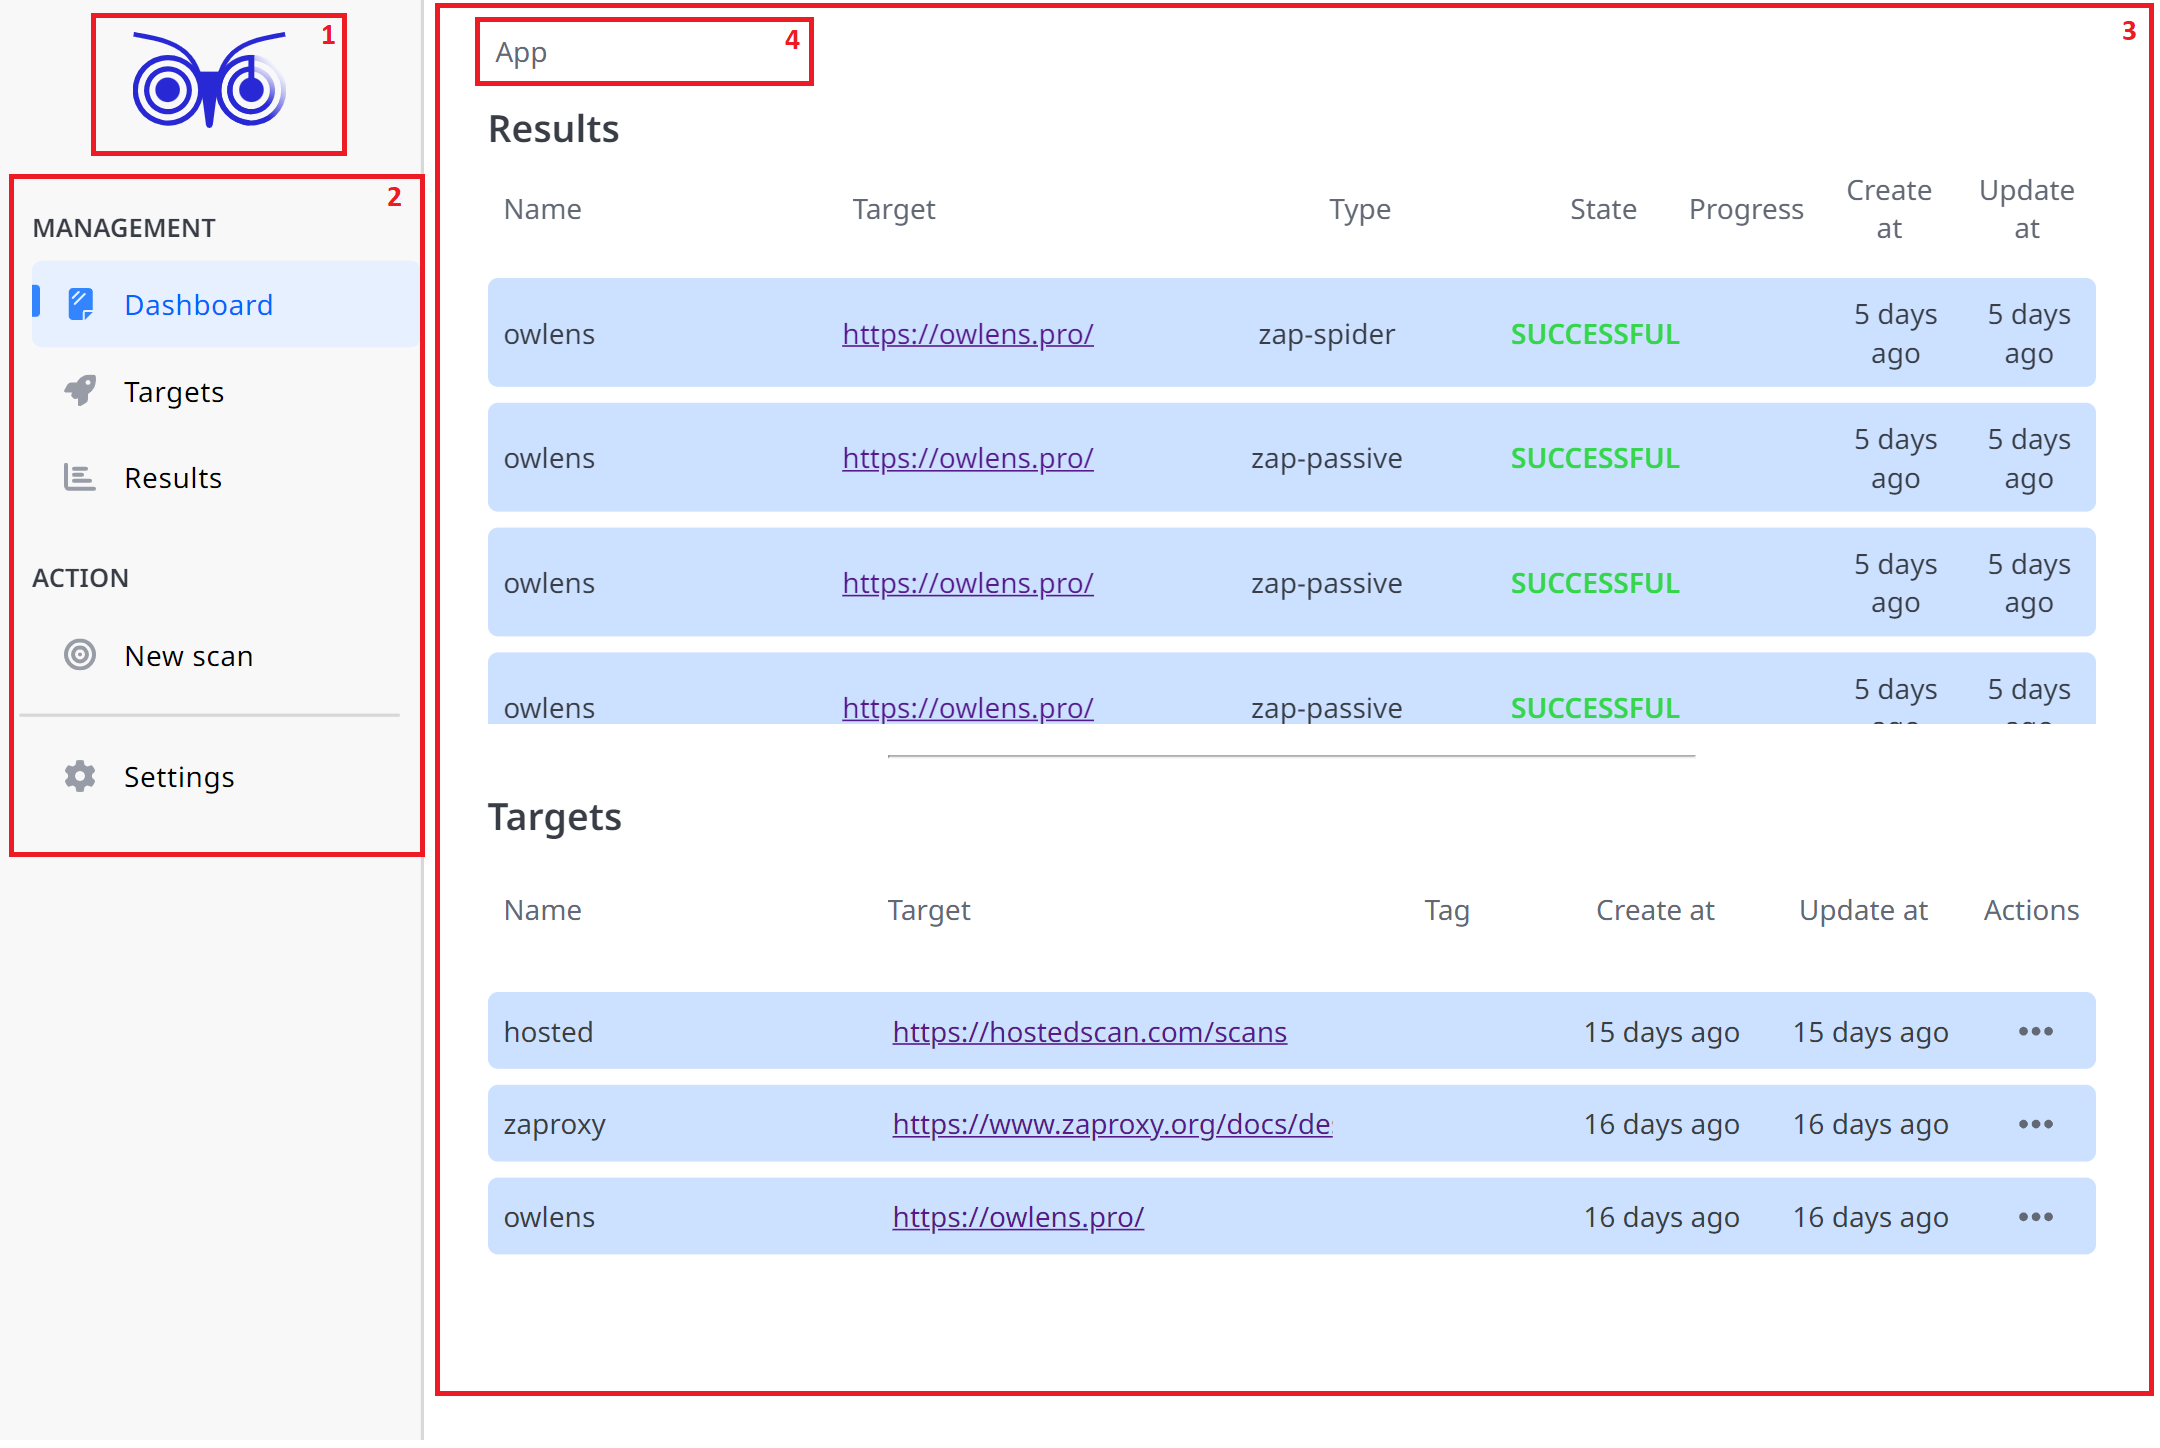
\includegraphics[width=\textwidth]{applied-thesis-chapters/chapter-3/Màn hình ứng dụng.png}
      \caption{Màn hình ứng dụng}
      \label{fig:MHUngDung}
\end{figure}

Bảng mô tả giao diện màn hình ứng dụng, bảng \ref{tab:MTUngDung}:

\begin{tabularx}{\textwidth}{|>{\hsize=.15\hsize\centering\let\newline
      \\\arraybackslash}X|>{\hsize=.30\hsize\raggedright\let\newline
      \\\arraybackslash}X|>{\hsize=.45\hsize\raggedright\let\newline
      \\\arraybackslash}X|}
      \hline
      \thead{STT}
       & \thead{Tên thành phần}
       & \thead{Mô tả}
      \\
      \hline
      1
       &
      Logo
       &
      Logo của ứng dụng Owlens. Người dùng có thể chọn vào logo để quay lại màn hình chính của ứng dụng cũng là màn hình của tùy chọn “Dashboard“.
      \\
      \hline
      2
       &
      Bảng tùy chọn
       &
      Người dùng có thể chuyển đổi giữa các bảng điều khiển bằng khác nhau tương ứng với các tuỳ chọn có trong bảng tùy chọn.
      \\
      \hline
      3
       &
      Bảng điều khiển
       &
      Bảng hiển thị các nội dung khác nhau tương ứng với các tùy chọn đang được chọn khác nhau.
      \\
      \hline
      4
       &
      Thanh truy vết địa chỉ
       &
      Cho phép người dùng theo dõi vị trí hiện tại trong ứng dụng và di chuyển lại truy vết trước đó.
      \\
      \hline
      \caption{Mô tả giao diện màn hình ứng dụng}
      \label{tab:MTUngDung}
\end{tabularx}

\section{Sơ đồ phần mềm hệ thống}

\subsection{Sơ đồ use case}

\tab Hình \ref{fig:UseCase} mô tả sơ đồ Use Case của hệ thống.

\begin{figure}[H]
      \centering
      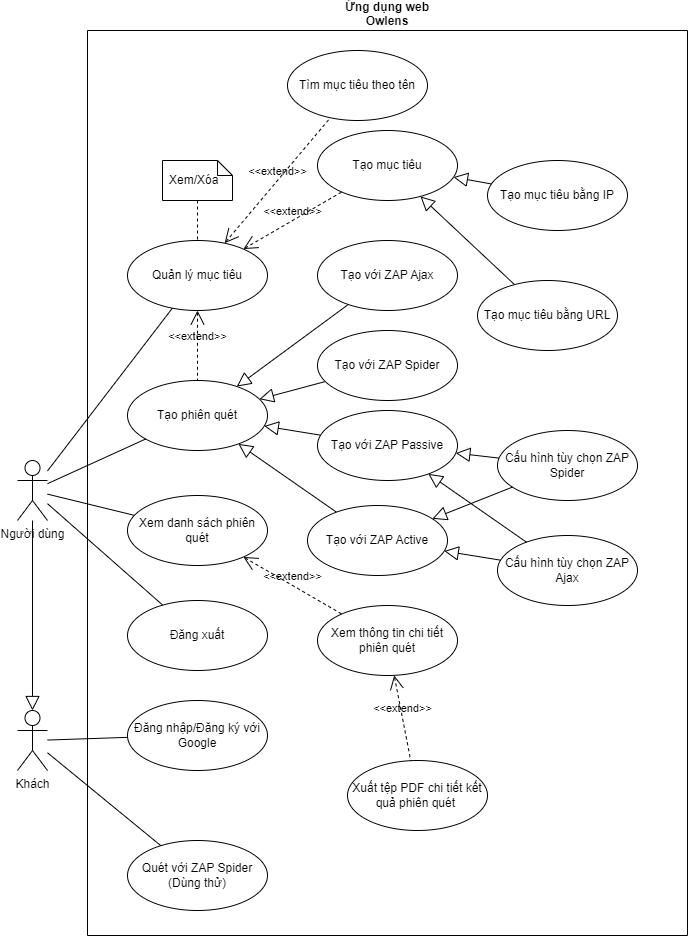
\includegraphics[width=\textwidth]{applied-thesis-chapters/chapter-3/Sơ đồ Use Case.png}
      \caption{Sơ đồ Use Case}
      \label{fig:UseCase}
\end{figure}

Bảng \ref{tab:UseCase} mô tả cho sơ đồ Use Case của hệ thống

\begin{tabularx}{\textwidth}{|>{\hsize=.15\hsize\centering\let\newline
      \\\arraybackslash}X|>{\hsize=.30\hsize\raggedright\let\newline
      \\\arraybackslash}X|>{\hsize=.45\hsize\raggedright\let\newline
      \\\arraybackslash}X|}
      \hline
      \thead{STT}
       & \thead{Use Case}
       & \thead{Mô tả}
      \\
      \hline
      1
       &
      Đăng nhập/Đăng ký với Google
       &
      Người dùng khách có thể đăng nhập vào hệ thống bằng tài khoản Google, nếu tài khoản của người dùng đăng nhập lần đầu sẽ được ghi nhận như đăng ký và đăng nhập cùng lúc
      \\
      \hline
      2
       &
      Quét với ZAP Spider (Dùng thử)
       &
      Người dùng khách có thể sử dụng thử chức năng quét với ZAP Spider. Vì là khách nên kết quả quét chỉ được hiển thị chứ không lưu vào hệ thống
      \\
      \hline
      3
       &
      Quản lý mục tiêu
       &
      Người dùng đã đăng nhập có thể xem danh sách mục tiêu, tạo và xóa các mục tiêu. Khi xem danh sách mục tiêu người dùng có tìm mục tiêu theo tên. Khi tạo mục tiêu, người dùng có thể tạo hai loại mục tiêu: mục tiêu bằng URL và mục tiêu bằng IP
      \\
      \hline
      4
       &
      Tạo phiên quét
       &
      Người dùng đã đăng nhập có thể tạo phiên quét mới từ các mục tiêu đã tạo. Các phương thức của phiên quét người dùng có thể chọn là: ZAP Spider, ZAP Ajax, ZAP Passive, ZAP Active. Ngoài ra, khi tạo các phiên quét bằng ZAP Passive hay ZAP Active, người dùng có thể chọn cấu hình loại khám phá (explore type) là ZAP Spider hoặc ZAP Ajax (mặc định là ZAP Spider)
      \\
      \hline
      5
       &
      Xem danh sách phiên quét
       &
      Người dùng đã đăng nhập có thể xem danh sách phiên quét. Danh sách phiên quét hiển thị thông tin chung của các phiên quét. Người dùng có thể chọn mục trong bảng để xem thông tin chi tiết của phiên quét. Trong màn hình của thông tin chi tiết phiên quét, người dùng có thể chọn xuất kết quả quét ra tệp PDF.
      \\
      \hline
      6
       &
      Đăng xuất
       &
      Người dùng đã đăng nhập có thể đăng xuất phiên đăng nhập của mình khỏi hệ thống
      \\
      \hline
      \caption{Mô tả sơ đồ Use Case}
      \label{tab:UseCase}
\end{tabularx}

\subsection{Sơ đồ cơ sở dữ liệu}

Hình \ref{fig:Database} mô tả sơ đồ cơ sở dữ liệu của hệ thống.

\begin{figure}[H]
      \centering
      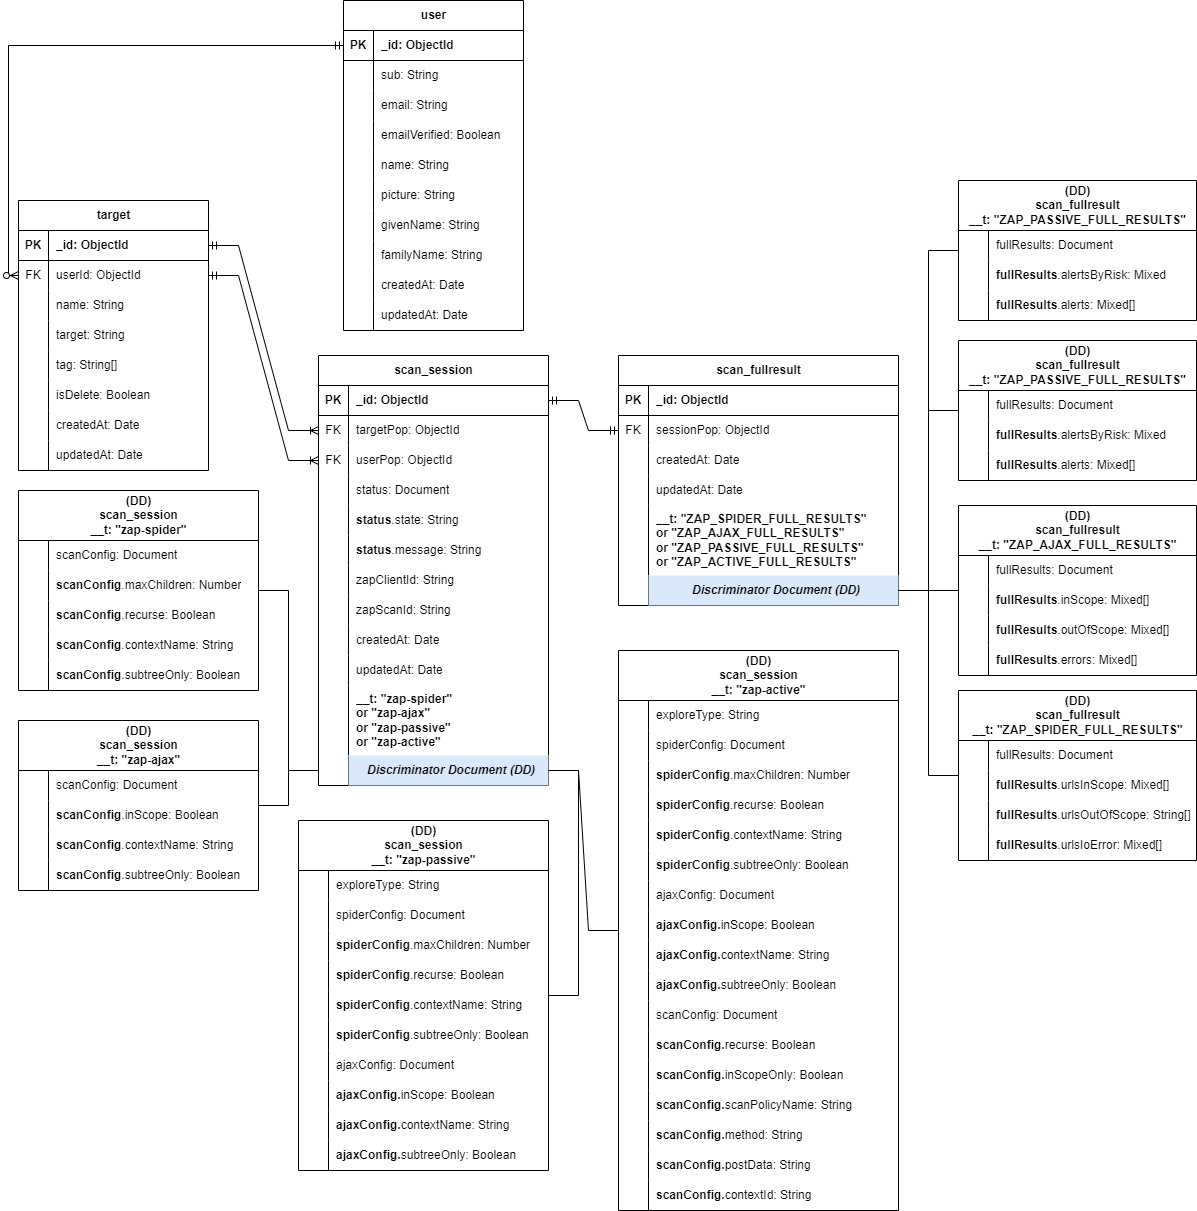
\includegraphics[width=\textwidth]{applied-thesis-chapters/chapter-3/Sơ đồ cơ sở dữ liệu.png}
      \caption{Sơ đồ cơ sở dữ liệu}
      \label{fig:Database}
\end{figure}